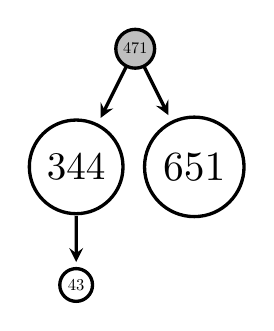
\begin{tikzpicture}[scale=3]
\tikzset{
	node/.style={circle,inner sep=1mm, draw,very thick,black,fill=white,text=black},
	smallestNode/.style={circle,inner sep=1mm, draw,very thick,black,fill=lightgray,text=black},
	arrow/.style={very thick,black,shorten >=2pt,-stealth},
}

	\node [smallestNode, scale=0.585590] (1) at (0.000000, 1.000000)	{471};
	\node [node, scale=1.412190] (2) at (-0.250000, 0.500000)	{344};
	\node [node, scale=0.598089] (3) at (-0.250000, 0.000000)	{43};
	\node [node, scale=1.500000] (4) at (0.250000, 0.500000)	{651};
	\path [arrow] (1) edge (2);
	\path [arrow] (1) edge (4);
	\path [arrow] (2) edge (3);

\end{tikzpicture}
